\documentclass[a4paper]{article}
\usepackage{pgfplots}
\usepgfplotslibrary{fillbetween}

\pgfplotsset{compat=1.9}


\begin{document}
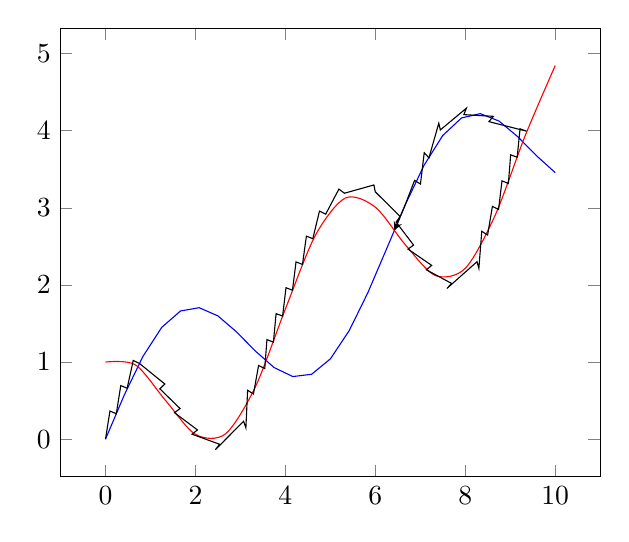
\begin{tikzpicture}
\begin{axis}[domain=0:10]

\addplot[name path=first,blue] 
	{sin(deg(x)) + 2/5*x};

\addplot[name path=second,red,
	samples=16,smooth] 
	{cos(deg(1.2*x)) + 2/5*x};

\draw[black,-stealth,
	decorate,decoration={
		saw,
		post=lineto,
		post length=10pt},
	intersection segments={	
		of=first and second,
		sequence={A0 -- B1 -- B2 
			-- B3 -- A3[reverse]}
	},
];

\end{axis}
\end{tikzpicture}

\end{document}


